\section{Datenbank / back end / cronjobs}
In diesem Kapitel wird aufgezeigt welche Änderungen an der Datenbank vorgenommen werden und wo diese überall zum Einsatz kommen. Zudem wird aufgezeigt, wie diese zusätzlichen Anwendungen entwickelt wurden. Vor der Umstrukturierung der Datenbank waren die Tabellen unübersichtlich aufgebaut. Nach der Umstrukturierung soll die Datenbank primär für folgende Aufgaben ausgelegt sein:\\
\begin{itemize*}
\item API
\item Dreitage Rückschau der verschiedenen Sensoren
\item Historische Daten
\end{itemize*}

Die Aufgabe der Datenbank ist es, den Umgang mit den Daten einfacher zu gestalten. Sei es in Bezug auf die Aufbereitung der historischen Daten oder für den Aufbau der API, welche einfach erweiterbar sein soll.



%% ############################################################################
%% Unterkapitel
%% ############################################################################
\subsection{Datenerfassung}
% Ueberischt über alle Kanäle -> was wird wie erfasst

\begin{figure}[htbp!]
  \fbox{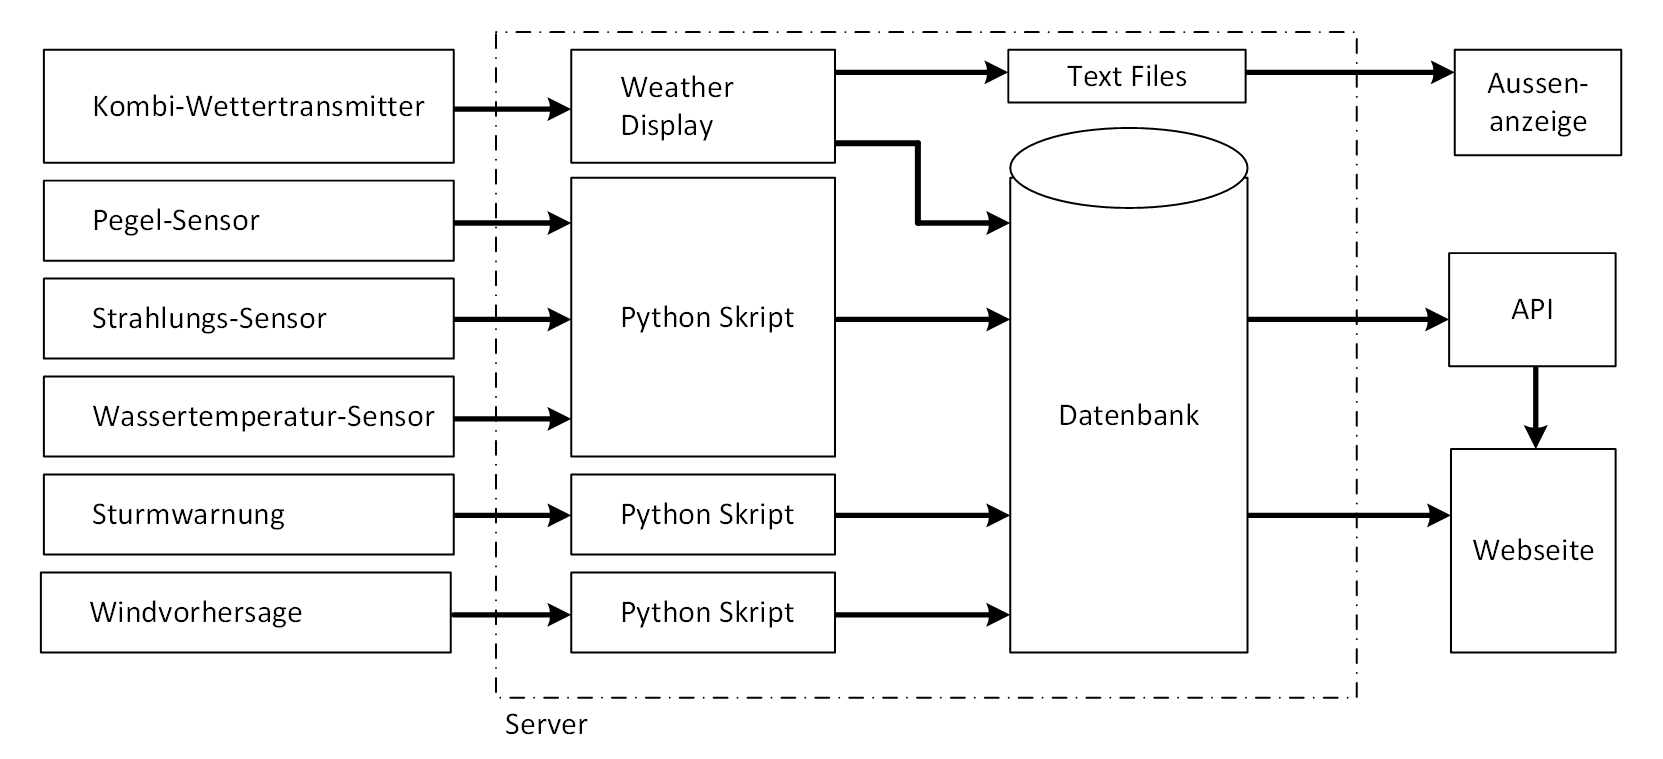
\includegraphics[width=\textwidth-2\fboxsep-2\fboxrule]{img/datenerfassung}}
	\centering
	\caption{Datenerfassung}
	\label{img:datenerfassung}
\end{figure}




\subsubsection{Erfassung der Daten des Wetter-Transmitters}
Die Daten des Wetter-Transmitters werden weiterhin von WeatherDisplay über eine virtuelle serielle Schnittstelle abgerufen sowie aufbereitet. Damit die Daten im Minutentakt in der Datenbank gespeichert werden. Für die Umgestaltung der Datenbank wurde auch die Konfiguration im WeatherDisplay angepasst. \Diskussionspunkt{Bild Weatherdisplay Konfiguration} In der Konfiguration können die Datenpunkte welche eingetragen werden sollen selektiert werden. \Diskussionspunkt{Weitere Konfigmöglichkeiten aufzeigen}

Kann ein Datenbankeintrag nicht erstellt werden, weil es zu wenig Einträge hat oder aus anderen Gründen wird dies, wie später im Kapitel Funktionsüberwachung mit Mail-Service \ref{kap:Funktionsüberwachung}, beschrieben im Cronjob abgefangen.

\subsubsection{Einlesen von Pegel- und Strahlungsmesswerten}
Wassertemperatur, Strahlungssensor und Pegelsenoren sind alle an einem Web-IO angeschlossen, welche die analogen Werte per Web-Schnittstelle zur Verfügung stellt. Die Abfrage erfolgt einmal pro Minute durch ein Python-Skript, wie in Listing \ref{lst:webIo} dargestellt. Der URL-Request wird mittels cURL ausgeführt. Die Abfrage ist für alle genannten Sensoren die gleiche, nur die URL unterscheidet sich je nach Sensor. Die Abfragen sind nach dem try... catch - Prinzip aufgebaut, sodass das Skript weiterläuft auch wenn vom Web-IO keine Antwort eintrifft.

\begin{lstlisting}[label=lst:webIo,caption=Python-Script zur Web-Abfrage des Pegel-Messwerts, language=python, style=py]
try:
    buffer = StringIO()
    c = pycurl.Curl()
    c.setopt(c.URL, 'http://webcam.wetter-arbon.ch:50506/single1')
    c.setopt(c.WRITEDATA, buffer)
    c.perform()
    c.close()
    requestMeasurement = buffer.getvalue()
\end{lstlisting}


\subsubsection{Abgreifen der Sturmwarndaten} % screen scrapping
Die Sturmwarndaten werden periodisch mittels Python-Skript ausgelesen. Als Web-Scrapper kommt die Python-Bibliothek \href{https://www.crummy.com/software/BeautifulSoup/}{\emph{BeautifulSoup}} zum Einsatz. Das Auslesen von Webseiten wird auch \emph{web scraping} genannt. Die Idee dahinter ist, die gewünschte Information auf Grund ihrer Element-Bezeichnung (\texttt{<td>}), ihres Attributs (\texttt{class="titelfett"}) oder Hierarchistufe (\texttt{tr:nth-of-type(4)}) eindeutig zu identifizieren. Um diese eindeutige Identifikation herauszufinden wurde das Google Chrome-Plugin \href{https://selectorgadget.com/}{\emph{SelectorGadget }} verwendet. Listing \ref{lst:kttgCrawler} zeigt die gesamte Abfrage. Darin ist das Problem dieser Methode gut erkennbar. Ändert die URL oder die Bezeichung bzw. Struktur der Seite, liefert das Skript nicht mehr die gewünschten Daten. Da das Web-Scrapping jedoch die einzige kostenlose Möglichkeit darstellt um die Daten zu erhalten, muss dieses Risiko akezptiert werden.


\begin{lstlisting}[label=lst:kttgCrawler,caption=Web-Scrapper für die Sturmwarndaten, language=python, style=py]
page = requests.get('http://www.kttg.ch/kapo/htm/stwarn.shtml')
soup = BeautifulSoup(page.text, 'html.parser')

# Einschaltzeit auslesen
soup.select('table tr:nth-of-type(4) td'):

# Status auslesen
soup.select('.titelfett strong'):
\end{lstlisting}


\subsubsection{Windvorhersagedaten}
Die Abfrage der Datenban stellt sich als recht kompliziert heraus. Sodass entschieden wurde eine VIEW einzusetzten. Diese wird dynamisch bei Aufrufen erzeugt und enthält die gewünschten Daten. Der SQL-Befehl für die Erzeugung der VIEW ist vereinfacht in Listing \ref{lst:viewForecast} aufgeführt. Primär gibt es zwei Bediungungen. Erstens sollen nur die Dreitageverhersagewerte verwendet werden und zweitens sollen die Vorhersagewerte verwendet werden, die am nächsten bei der aktuellen Zeit liegen. Da das Vorhersageintervall 3 Stunden beträgt ist die Verhersage maximal 1.5 Stunden verschoben.

%View erstellen
\begin{lstlisting}[label=lst:viewForecast,caption=Erzeugung der VIEW für den Forecast-Vergleich, language=SQL, style=htmlcssjs]
SELECT *
FROM 'tblcompwindfinder'
WHERE
(datetime + interval 3 day) <= now() #heute vor drei Tagen
AND
abs(timediff(datetime,now())) <= 13000) #innerhalb +/- 1.5h
ORDER BY datetime DESC
LIMIT 3
\end{lstlisting}



%% ############################################################################
%% Unterkapitel
%% ############################################################################
\subsection{Datenspeicherung}
Für die Datenspeicherung stellt Hostpoint, der Webhosting-Provider der Wetterstation, seinen Kunden eine MariaDB Version 10.1 mit dem Administrationstool phpMyAdmin zur Verfügung. MariaDB ist eine relationales Open-Source-Datenbankverwaltungssystem und basiert auf MySQL.

Die Datenbank wurde komplett neu aufgebaut. Im Folgenden werde die einzelnen Tabellen und deren Struktur erklärt.

%Für die Umstrukturierung wurde von der Methodik aus dem Artikel Grundlagen und Entwurf \cite{Datenbanken:GrundlagenUndEntwurf:VeikkoKrypczyk} gebrauch gemacht.
%Wie in Introduction to relational Databases \cite{IntroductionToRelationalDatabases:MariaDB} beschrieben wird,

\subsubsection{Aufbau und Inhalt der Datenbank}
Die Datenbank besteht aus mehreren Tabellen mit unterschiedlichem Inhalt. Die Auflistung sämtlicher Tabellen mit einer Beschreibung des Inhalts befindet sich in Tabelle\,\ref{table:dbtabellen}. Die obersten vier Tabellen werden zur Speicherung der Messwerte/Zusatzinformationen verwendet. Anschliessend kommen die drei Tabellen für die historischen Daten und zum Schluss zwei Tabelle, die für den Benachrichtungsservice und die Webcam benötigt werden.
%\Diskussionspunkt{Warum wurde keine zweite DB für Benachrichtigungsservice und Webcam erstellt? Zweite DB mit igwetter_Services?}

% Datenbank-Tabellen
\begin{table}[htbp!]
  \setlength\extrarowheight{3pt} % for a more "open" look
  \begin{tabularx}{\textwidth}{|>{\RaggedRight\hspace{0pt}}p{4.5cm}|X|}

  \hline
  %\textbf{Tabelle}
  & \bfseries Beschreibung \\

  \hline
  \textbf{tblwettertransmitter}
  & Messwerte des Wettertransmitters \\

  \hline
  \textbf{tblextsensors}
  & Messwerte der Sensoren (Bsp. Pegel) \\

  \hline
  \textbf{tblmisc}
  & Daten vorn Dritten (Bsp. Sturmwarnung) \\

  \hline
  \textbf{tblcompwindfinder}
  & Windvorhersagewerte von Windfinder \\

  \hline
  \hline
  \textbf{tbldatemaster}
  & Daten vom 1.1.2015 bis 31.12.2035 im Minutenabstand \\

  \hline
  \textbf{tblhistorical}
  & Messwerte zusammengefasst auf 1Eintrag/h \\

  \hline
  \textbf{tblwaterlevelhistorical}
  & Pegelwerte von 1953 bis heute \\

  \hline
  \hline
  \textbf{tblnotifications}
  & Abos des Benachrichtigungsservices \\

  \hline
  \hline
  \textbf{tblqueue}
  & Warteschlange der Webcam \\

  \hline
  \end{tabularx}
  \caption{Datenbanktabellen und deren Inhalt}
  \label{table:dbtabellen} % label muss NACH caption stehen!!!!
\end{table}

\noindent
Die Tabellen haben untereinander keine Verknüpfung (Relation), sondern sind alle eigenständig. Das einzige, was sie verbindet ist der Zeitstempel des Messzeitpunkts. Es wird deshalb auf die Erstellung eines ER-Modells, wie in Datenbanken Grundlagen und Design \cite{FrankGeisler2011mitpu} beschrieben, verzichtet. In Abbildung\,\ref{img:tabellenstruktur} ist beispielhaft die Struktur der Tabelle \emph{tblextsensors} aufgeführt. Als Primärschlüssel wird jeweils der Zeitstempel des Messzeitpunkts verwendet. Da der Primärschlüssel ein UNIQUE-Wert ist, wird verhindert, dass es zwei Einträge mit dem selben Zeitstempel gibt. Das komplette relationale Datenmodell mit allen Entitäten und deren Attributen befindet sich in Anhang\,\ref{anhang:relationalesDatenbankmodell}.

\begin{figure}[htbp!]
  \fbox{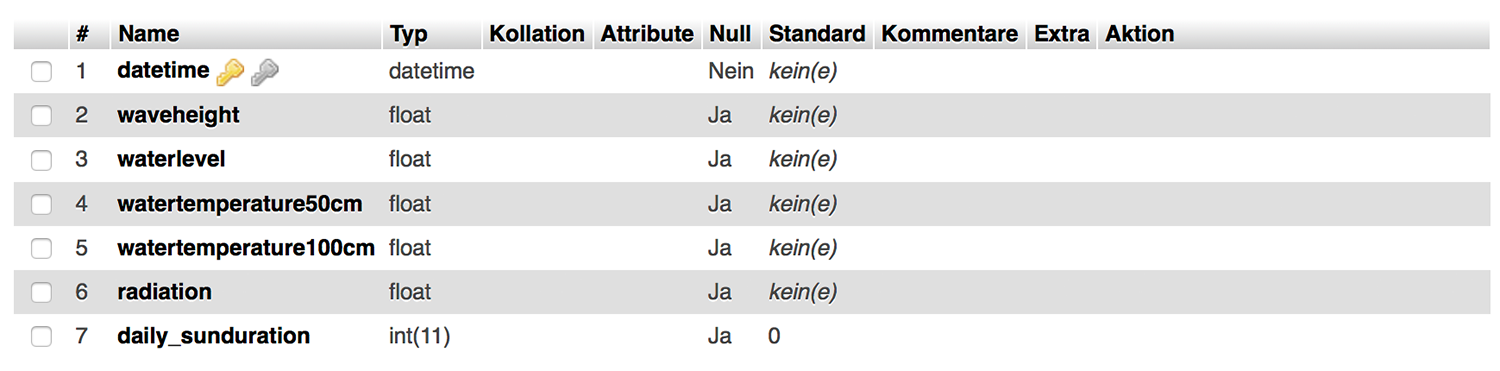
\includegraphics[width=\textwidth-2\fboxsep-2\fboxrule]{img/tabellenstruktur}}
	\centering
	\caption{Struktur der Tabelle \emph{tblextsensors}}
	\label{img:tabellenstruktur}
\end{figure}

%Die Normalisierung ist, wie in Datenbanken Grundlagen und Design \cite{FrankGeisler2011mitpu}, ein Prozess mit deren Hilfe die Datenbankstruktur optimiert wird und hilft dabei Datenredundanzen zu vermeiden. Da bei der Datenbank nur das Datum redundant ist, ist eine Normalisierung nicht notwendig.
%Das relationale Datenmodell unterscheidet sich in der Struktur nicht bedeutend vom ER-Modell. Der Unterschied  ist, dass die Primärschlüssel und die Datentypen festgelegt werden. Die sogenannten Schlüssel sind im relationalen Datenmodell auch ein wichtiges Merkmal. Bei zukünftigen Datenbankeinträgen sind entscheidend die Schlüssel, so kann verhindert werden, dass für einen gewissen Zeitpunkt nochmals Datensätze geschrieben werden.
%Die drei konzipierten Tabellen konnten wie gewünscht umgesetzt werden. Der Code für die Umsetzung der Tabellen, kann aus dem Anhang \ref{anhang:Datenbankcode} entnommen werden.\\


\subsubsection{Erstellen der historischen Datenbank , Ausdünnen,  LEFT JOIN}
Bei der Wetterstation fallen pro Minute 65 Datenpunkte vom Wettertransmitter an, sowie 4 Datenpunkte von den externen Sensoren.

% Wie funktioniert das Zusammenfassen der Daten -> SQL-Befehle
% Abbildung hinzufügen wo Script sichtbar Ist



Die Herausforderung bei der Umsetzung war es, dass die historische Tabelle, welche aus den beiden Tabellen tblwettertransmitter und tblextsensors bestehen, mittels einer Query zusammenzubringen.



Das Problem war die Zeit. Die Daten des Wettertransmitters werden Konfigurationsbedingt, nicht auf die Minute genau, sondern 31 Sekunden später geschrieben. Bei einem LEFT JOIN, welches über die Zeit geht, werden auch die Sekunden angeschaut. Nach mehreren gescheiterten Versuchen, ist es anschliessend gelungen, eine passende Query wie in \ref{lst:LeftJoinQuery} zu entwickeln.

Zudem wird eine historische Tabelle erstellt, diese soll, die zu stündlich aufbereiteten Daten aus den beiden Tabellen enthalten. Um die historische Tabelle ohne Ausfälle zu füllen wird eine Tabelle entstehen, welche alle Zeitstempel von 2015 bis 2030 beinhaltet. Welche Datenpunkte übernommen werden, kann aus dem Anhang \ref{anhang:Datenbankschema} entnommen werden.\\

Beim Modell der historischen Daten sieht das ganze anders aus (siehe Abb. \ref{img:ER_Modell historische Daten}). Hier beinhaltet jeder Zeitstempel, den Median, sowie die Extremwerte der Daten vom Wettertransmitter und die der externen Sensoren.

Zusätzlich sollen die Daten, welche weiterhin im Minutentakt geschrieben werden, so aufbereitet werden, dass Benutzer auf der neu erstellen historischen Webpage die Wetterdaten der vergangenen Jahre einsehen können.


\begin{lstlisting}[label=lst:LeftJoinQuery,caption=Json Struktur, language=JavaScript, style=htmlcssjs, mathescape]
SELECT * FROM `DateMaster`
LEFT JOIN `tblwettertransmitter`
ON MINUTE(dt) = MINUTE(datetime)
WHERE ((`DateMaster`.`dt` > (now() - interval 2 hour))
AND((`tblwettertransmitter`.`datetime` > (now() - interval 2 hour))
AND (hour((now() - interval 1 hour)) = hour(`tblwettertransmitter`.`datetime`)))
AND (hour((now() - interval 1 hour)) = hour(`DateMaster`.`dt`))
AND (`DateMaster`.`dt` < now()))
order by `DateMaster`.`dt` desc
\end{lstlisting}





%% ############################################################################
%% Unterkapitel
%% ############################################################################
\subsection{Datenbanksicherheit}
\subsubsection{Speicherplatz}
Bevor sich Gedanken um die Datensicherheit gemacht werden, sollten die Bedingungen an den Speicherplatz klar sein. Während der Laufzeit werden grosse Mengen an Daten in die Datenbank geschrieben. Vor der Neukonzipierung werden täglich 1440 Datensätze gespeichert. Das bedeutet jede Minute einen Datensatz. Ein Datensatz beinhaltet 65 Einträge, die gesamte relevante Datenbank igwetter wettertest benötigt (Stand 2018-04-24) 323.2  Mb. Die Tabelle wx data, beinhaltet die Minutenwerte des Wettertransmitters, benötigt davon (Stand 2018-04-24) 311.9 Mb, daraus erfolgt das ein Datensatz ca 0.025 Mb benötigt. Für den Speicherplatz, welcher 50 Gb bietet, stellt dies kein Problem dar. Hochrechnet reicht der Platz für die kommenden 45 Jahren.

\subsubsection{Angriffssicherheit}
Bei der Recherche nach Datenbanksicherheit taucht immer wieder das Wort Injection auf. Laut den OWASP top 10, eine Liste welche die wichtigsten Schwachstellen aufzeigt, ist die SQL-injection in 2017 auf dem Platz 1. Was ist den eigentlich SQL Injection? SQL injection ist eine Methode eine Datenbankabfrage so zu manipulieren, dass der Angreifer im schlimmsten Fall auf die gespeicherten Daten des Administators kommt. Ein anderes Beispiel wäre, dass die Angreifer an die Daten der Benutzer eines Online-Shops mit Kreditkartendaten oder ähnlichen sensitiven Daten kommen.
Weitere Fragen die zum Thema Dantenbanksicherheit auftauchen sind:
\begin{itemize}
\item Was für Arten von Daten beherbergt die Datenbank?
\item Hat es sensitive Daten?
\item Ist die Datenbank überhaupt ein potentielles Angriffsziel?
\item Wer sind die Benutzer der Datenbank?
\end{itemize}

Bei der Wetterstation Arbon, bestehen keine persönliche oder sicherheitsrelevante Daten in der Datenbank. Somit ist diese aus Sicht eines potentiellen Angriffes eher uninteressant. Dennoch sollten die Daten hinreichend geschützt sein, da es vor allem schade wäre wenn die Daten verloren gingen. Andererseits sollte der Server vor Missbrauch geschützt werden.

Die Zugriffe auf die Datenbank sind so gestaltet, dass nur Serverseitig darauf zugegriffen wird. Die Darstellung der Anzeigen auf der Webseiten werden über die API erstellt. Die API wiederum ist so aufgebaut, dass ein PHP-Skript auf dem Server die Daten aus der Datenbank abgreift und sie richtig formatiert. Somit kann sichergegangen werden, dass keine SQL-Injection möglich ist. Wie im Kapitel Daten der neuen Wetterstation mit Tableau \ref{kap:Tableau} erwähnt, müssen die Daten für das Tableau manuell übertragen werden. Dies bedeutet, dass für die historische Seite kein Datenbankzugriff notwendig ist.

\subsubsection{Backup}
Um die Datenbank gegen einen allfälligen Datenverlust zu sichern, ist ein Backup von wichtiger Bedeutung. Deswegen ist das Backup ein weiterer Aspekt gegen den Verlust von Daten. Hierbei sind folgende Fragen relevant:
\begin{itemize}
\item Welche Daten sollen gesichert werden?
\item Wie oft sollten die Daten gesichert werden?
\item Wie bzw. wo sollte das Backup gelagert werden?
\end{itemize}

Da alle Daten in der DB gleich relevant sind, sollten auch alle so behandelt werden und im Backup vorhanden sein. Dabei muss aber entschieden werden, ob ein tägliches Backup Sinn machen würde. Da die Wetterstation von einem Verein betrieben wird, ist es wichtig den Aufwand mit dem Ertrag zu vergleichen. Zusätzlich sollte das Backup nicht auf dem Server des Providers gespeichert werden, sollte etwas mit dem Server nicht in Ordnung sein, sind diese Daten auch weg. Deswegen ist es wichtig auch ein 'externes' Backup zu erstellen. Hostpoint bietet für das Backup verschiedene Varianten:
\begin{itemize}
\item Cronjob
\item Backup auf Knopfdruck
\item Kostenpflichtige Wiederherstellung aller Daten
\end{itemize}


Um den Aufwand klein zu halten, wird empfohlen ein monatliches Backup mit der Backup Funktion auf Knopfdruck zu erstellen und dieses auf einer Festplatte zu speichern (Abb. \ref{img:Backup_Funktion}).
\begin{figure}[h!]
  \fbox{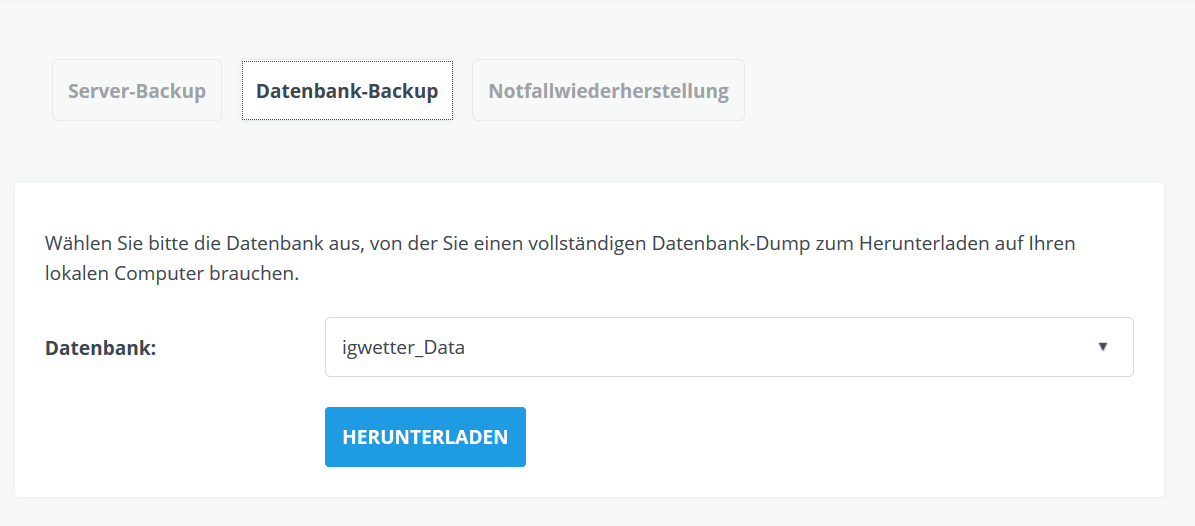
\includegraphics[width=\textwidth-2\fboxsep-2\fboxrule]{img/Backup_funktion}}
	\centering
	\caption{Backup auf Knopfdruck von Hostpoint}
	\label{img:Backup_Funktion}
\end{figure}
Sollte trotzdem mal das Backup nicht funktionierten oder vergessen gegangen sein, kann auf den Hostpoint-Service ( Abb.\ref{img:Notfallwiederherstellung}) züruck gegriffen werden. Diese erstellen selber ein tägliches Backup, welches für 100 Franken wieder eingespielt werden kann.
\begin{figure}[h!]
  \fbox{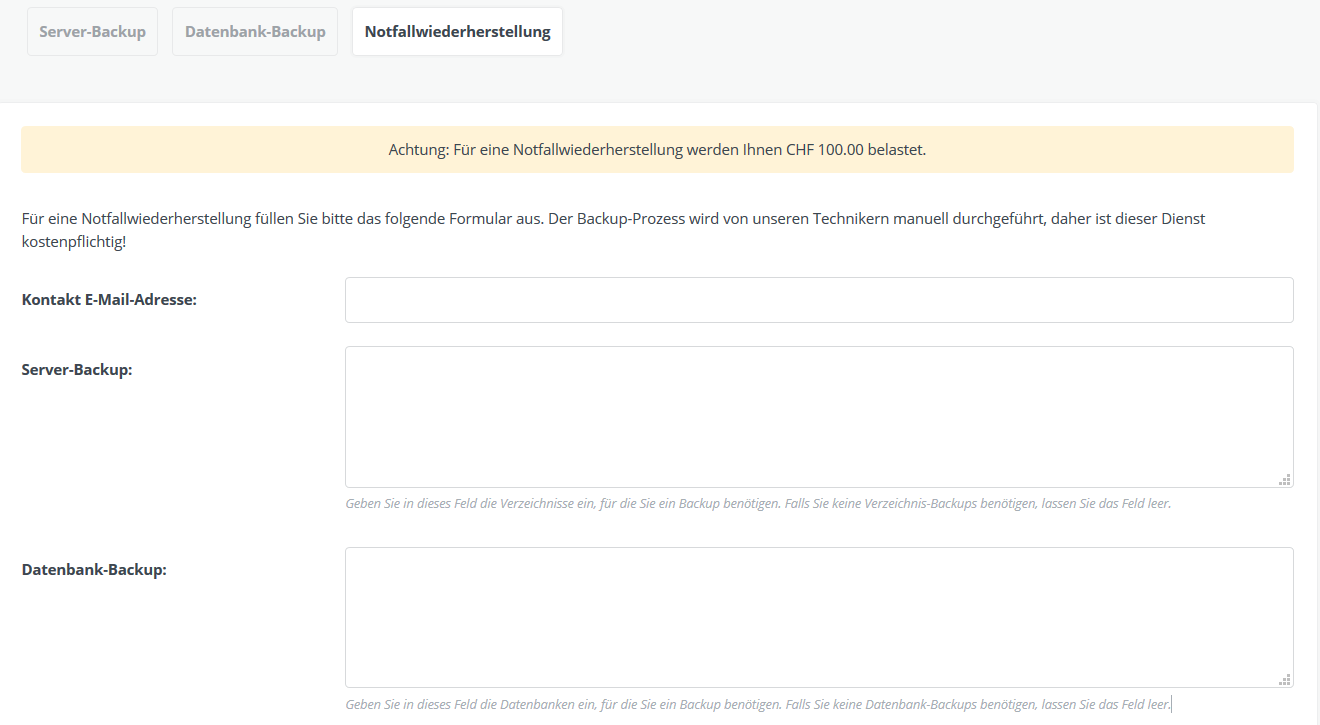
\includegraphics[width=\textwidth-2\fboxsep-2\fboxrule]{img/Notfallwiederherstellung}}
	\centering
	\caption{Notfallwiederherstellung von Hostpoint}
	\label{img:Notfallwiederherstellung}
\end{figure}
Somit können sich, davon ausgehend, dass Hostpoint einen guten Job macht Kosten für bspw. ein Cloudaccount gespart werden.

%% ############################################################################
%% Unterkapitel
%% ############################################################################
\subsection{Datenarchivierung}

In der Datenarchivierung werden die historischen Daten aufbereitet und komprimiert. Dafür ist wird von der historischen Tabelle gebrauch gemacht. Mittels einem Cronjob und dem in \ref{lst:LeftJoinQuery} codierten Left Join werden die Minuten Daten komprimiert. Anschliessend bestehen zwei Varianten:\\
\begin{itemize}
\item \textbf{Variante 1}\\
Die Daten aus den beiden Minutentabellen werden gelöscht, stehen somit nicht zu weiteren Zwecken zur Verfügung.
\item \textbf{Variante 2}\\
Die Daten aus den beiden Minutentabellen werden nicht gelöscht und können für spätere Anwendungen verwendet werden.
\end{itemize}

Da beim Server der Speicherplatz kein ausschlaggebender Punkt ist, wurde für die zweite Variante entschieden.


%% ############################################################################
%% Unterkapitel
%% ############################################################################
\subsection{Funktionsüberwachung mit Mail-Service}\label{kap:Funktionsüberwachung}
Um die Funktion der Software zu gewährleisten, sollte bei einem Absturz der Verantwortliche für die IG bei der IG benachrichtigt werden. Folgende Funktionen müssen bei einem Absturz eine Meldung geben.
\begin{itemize}
\item Einlesen Sensordaten extern
\item Einlesen Wettertransmitter Daten
\item Erstellung der stündlichen historischen Daten
\end{itemize}
Die Aufgezählten Funktionen werden alle bis auf das Einlesen der Wettertransmitter Daten über einen Cronjob ausgeführt. Hierfür bietet Hostpoint einen GUI Service, dass bei einem print() die Ausgaben per Mail an eine bestimmte Mailadresse gesendet werden (Listing \ref{lst:printfunction}). Für das Einlesen der externen Sensordaten sieht der Mailservice folgendermassen aus. Kann einer der Webservices vom Web-IO nicht erreicht werden, wird die folgende Mail generiert:\\
\begin{quote}
Es ist ein Problem mit (der Temperatur, dem Pegel, dem Strahlungssensor) aufgetreten. Exception: ...\\
\end{quote}
Je nach Sensor wird dieser genannt und das Problem welches aufgetreten ist. Beim Auslesen des Wettertransmitters ist diese Möglichkeit nicht direkt anwendbar. Hier wird beim erstellen der historischen Daten kontrolliert ob alle 60 Einträge der letzen Stunde vorhanden sind. Ist dies nicht der Fall, würde es bedeuten, dass das WeatherDisplay abgestürzt ist und neu gestartet werden muss. Die Meldung sieht folgendermassen aus:\\
\begin{quote}
Bitte starte das WeatherDisplay neu, es wurden nur (Anzahl Datensätze) Daten geschrieben.
\end{quote}

Auch beim schreiben in die historische Datenbank können Ausnahmen auftauchen. Ist dies der Fall wird folgende Meldung generiert:\\
\begin{quote}
Die historischen Daten können nicht geschrieben werden, es besteht folgendes Problem (Exception).
\end{quote}

Um diese Funktionen zu erstellen wird Gebrauch vom try, except Verfahren in Python gemacht. Zu Beginn wird der Code im try ausgeführt, tritt keine exception auf, wird das except übersprungen und der anschliessende Code ausgeführt. Tritt aber während dem try eine exception auf, wird der Code unterbrochen und der im except weitergeführt. Anschliessend wird der Code nach dem Exception Handling ausgeführt.\cite{ThePythonTutorial8.ErrorsAndExceptions:Python}

\begin{lstlisting}[label=lst:printfunction,caption=Beispiel für print Funktion, language=Python, style=py]
except Exception as e:
    print "Es ist ein Problem mit der Strahlungs Abfrage aufgetaucht: "
    print e
\end{lstlisting}

%% ############################################################################
%% Unterkapitel
%% ############################################################################
\subsection{Cron-Jobs}
Wie immer wieder in den vorherigen Kapitel erwähnt, werden viele Funktionen mit Cronjobs ausgeführt. Was ist ein Cronjob? Wie von Hostpoint \cite{Hostpoint:CronjobsEinrichten} dargestellt, werden Cronjob für wiederkehrende Abläufe verwendet. Anders formuliert, kann ein Script zu einem bestimmten Zeitpunkt automatisiert ausgeführt werden. Es wird angegeben zu welchem Zeitpunkt oder in welchem Intervall das Programm ausgeführt werden soll. Der Rest übernimmt dann anschliessend der Cronjob. In diesem Fall, das Auslesen der externen Sensordaten, das erstellen der historischen Daten und das auslesen der Sturmwarnung. Auf Hostpoint kann mittels Knopfdruck ein Cronjob erstellt werden. Dabei kann auch gleich konfiguriert werden, zu welcher Zeit ein Cronjob ausgeführt werden soll (Abb. \ref{img:ER_Modell Wettertransmitter}).

\begin{figure}[h!]
  \fbox{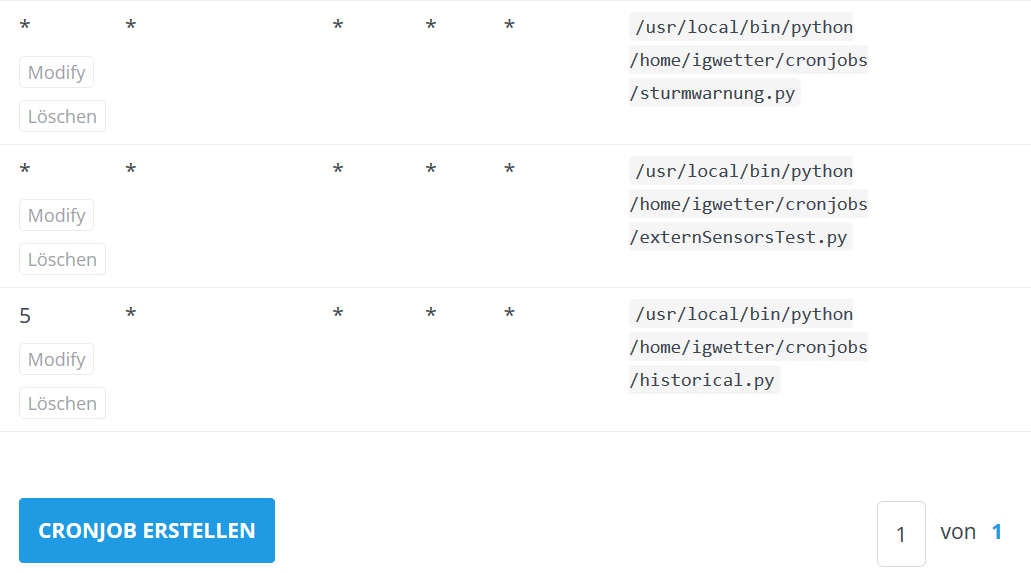
\includegraphics[width=\textwidth-2\fboxsep-2\fboxrule]{img/cronjob.png}}
	\centering
	\caption{Erstellen eines Cronjobs bei Hostpoint}
	\label{img:Cronjob}
\end{figure}

Die erwähnten Cronjob sind die wichtigsten, werden diese nicht durchgeführt, werden auch keinen Daten ausgelesen bzw. erstellt. Neben diesen drei Cronjobs bestehen noch zwei weitere. Diese lesen die Wettervorhersage für den Vergleich aus und schreiben die Daten in die Datenbank.

%% ############################################################################
%% Unterkapitel
%% ############################################################################
\subsection{Problematik Zeitumstellung}
Da in der Schweiz Sommer- und Winterzeit herrscht, besteht auch die Problematik der Zeitumstellung. Für die Datenbank besteht das Problem, dass die Tabellen nur einen Datumzeit enthalten dürfen. So entsteht die Problematik im Winter, da wenn die zurück gestellt wird doppelte Einträge entstehen. Wird in die historische Daten geschaut, fällt auf das diese Zeitumstellung nie berücksichtigt wurde. Zudem ist die Zeitumstellung in der Nacht, also für viele Benutzer eher uninteressant. Somit spielt es keine Rolle, dass die Daten bei der Zeitumstellung verloren gehen.




\subsection{DB-Nutzer Konzept}
welche Nutzer gibt es und welche Rechte haben sie -> theoretisch erklären
